\documentclass[12pt]{article}
\usepackage[english]{babel}
\usepackage[utf8]{inputenc}
\usepackage{amsmath, amssymb, amsthm}
\usepackage{graphicx}
\usepackage{hyperref}
\usepackage[margin=.75in]{geometry}
\usepackage{xcolor}
\usepackage{tikz}

\newcommand{\id}{\text{id}}
\newcommand{\od}{\text{od}}

\setlength{\topmargin}{0pt}
\setlength{\headsep}{0pt}
\textheight = 600pt

\title{Graph Theory \\ Homework 14}
\author{Ben Kallus and Ryan Friedman}
\date{Due Friday, April 16}

\begin{document}
\maketitle

\medskip\noindent\textbf{9.2} Proposition: A connected $k$-regular graph of order 12 embedded in the plane with 8 regions must be 3-regular.
\begin{proof}
    Let $G$ be a $k$-regular graph of order 12 embedded in the plane with 8 regions.
    Then, by Euler's Formula,
    \begin{align*}
        12 - \frac{12k}2 + 8 &= 2 \\
        \implies \frac{12k}2 &= 18 \\
        \implies k &= 3.
    \end{align*}

    Thus, $G$ is 3-regular.
\end{proof}

\newpage\noindent\textbf{9.6}

\textbf{(a)} Proposition: Every subgraph of a planar graph is planar.
\begin{proof}
    Let $G$ be a planar graph.
    Let $G'$ be a subgraph of $G$.
    Let $G''$ be a subgraph of $G'$.
    By Kuratowski's Theorem, no subgraph of $G$ is a subdivision of $K_5$ or $K_{3,3}$.
    Because $G'$ is a subgraph of $G$, $G''$ must also be a subgraph of $G$.
    Thus, $G''$ is not a subdivision of $K_5$ or $K_{3,3}$.
    Thus, $G'$ is planar.
\end{proof}

\textbf{(b)} Proposition: There exists a nonplanar graph with a planar subgraph.
\begin{proof}
    Note that $K_5$ is nonplanar.
    Consider the subgraph of $K_5$ induced by only one of its vertices.
    This graph is therefore isomorphic to $K_1$.
    Since the only subgraph of $K_1$ is $K_1$, and $K_1$ is not a subdivision of $K_5$ or $K_{3,3}$, $K_1$ is planar.
    Thus, $K_5$ has a planar subgraph.
\end{proof}

\textbf{(c)} Proposition: There exists a nonplanar graph does not have any nonplanar proper subgraphs.
\begin{proof}
    Note that $K_{5}$ is nonplanar.
    Because each vertex in $K_5$ is in a position symmetric to each other vertex in $K_5$.
    Thus, $K_5-uv \cong K_5-xy$ for all $u,v,x,y \in V(K_5)$.
    Let $u,v \in V(K_5)$.
    Consider the graph $K_5-uv$:
    \begin{center}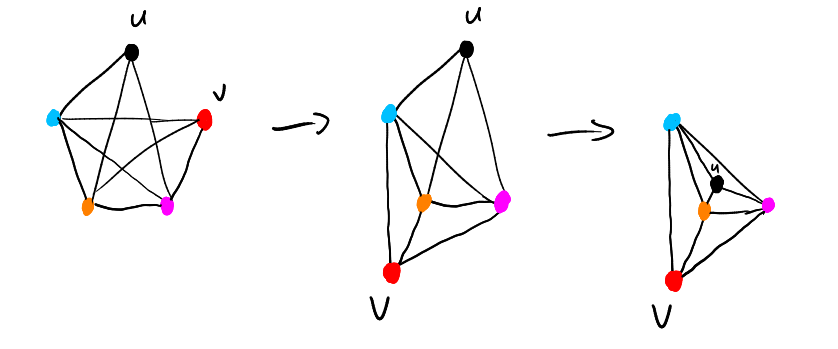
\includegraphics[scale=.7]{96c.png}\end{center}
    Clearly, $K_5 - uv$ is planar.
    Thus, by \textbf{(a)}, all subgraphs of $K_5$ are planar.
\end{proof}

\textbf{(d)} Proposition: There exists a nonplanar graph that does not contain $K_5$ or $K_{3,3}$ as a subgraph.
\begin{proof}
    Let $G$ be defined by the following drawing:
    \begin{center}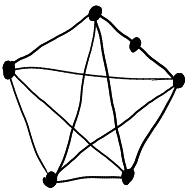
\includegraphics{96d.png}\end{center}
    Removing any edge from $G$ reduces the number of vertices with degree at least 4 in $G$ to less than 5, so $G$ cannot have $K_5$ as a subgraph.
    Because $G$ has only 5 vertices of degree at least 3, $G$ cannot have $K_{3,3}$ as a subgraph.
    Note that $G$ is nonplanar, because it is a subdivision of $K_5$; this is made clear by transforming $G$'s degree-2 vertex and its edges into a single edge.
    Thus, $G$ is a nonplanar graph that does not contain $K_5$ or $K_{3,3}$ as a subgraph.
\end{proof}

\textbf{(e)} Proposition: There exists a nonplanar graph of order $n$ and size $m$ such that $m \leq 3n - 6$.
\begin{proof}
    The graph of Figure 9.16, from \textbf{9.10} satisfies this condition.
\end{proof}

\textbf{(f)} Proposition: There exists a nonplanar graph with one or more triangles that contains no subdivision of $K_5$ as a subgraph.
\begin{proof}
    Let $G$ be defined by the following drawing:
    \begin{center}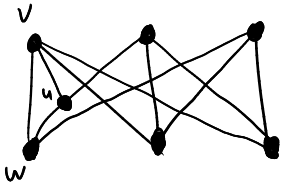
\includegraphics{96f.png}\end{center}
    Clearly, $G$ contains the triangle $uvw$.
    However, $G - uv$ is clearly a subdivision of $K_{3,3}$, so $G$ is nonplanar.
\end{proof}

\newpage\noindent\textbf{9.8} Proposition: $K_4 \times K_2$ is nonplanar.
\begin{proof}
    The following shows the construction of $G'$, a subgraph of $K_4 \times K_2$, then shows that $G'$ is a subdivision of $K_5$:
    \begin{center}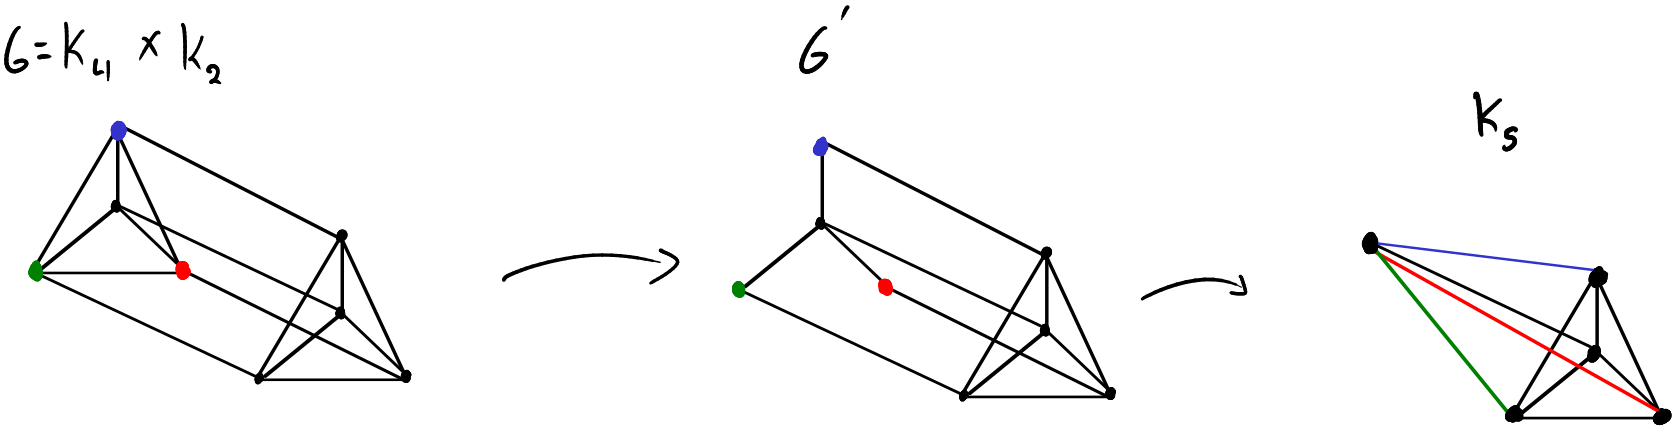
\includegraphics[scale=.4]{98.png}\end{center}
    Thus, by Kuratowski's Theorem, $K4 \times K_2$ is nonplanar.
\end{proof}


\newpage\noindent\textbf{9.10} Proposition: The graph of Figure 9.16 is nonplanar.
\begin{proof}
    The following figure shows the construction of a a subgraph of the graph of Figure 9.16, then shows that that subgraph is a subdivision of $K_5$:
    \begin{center}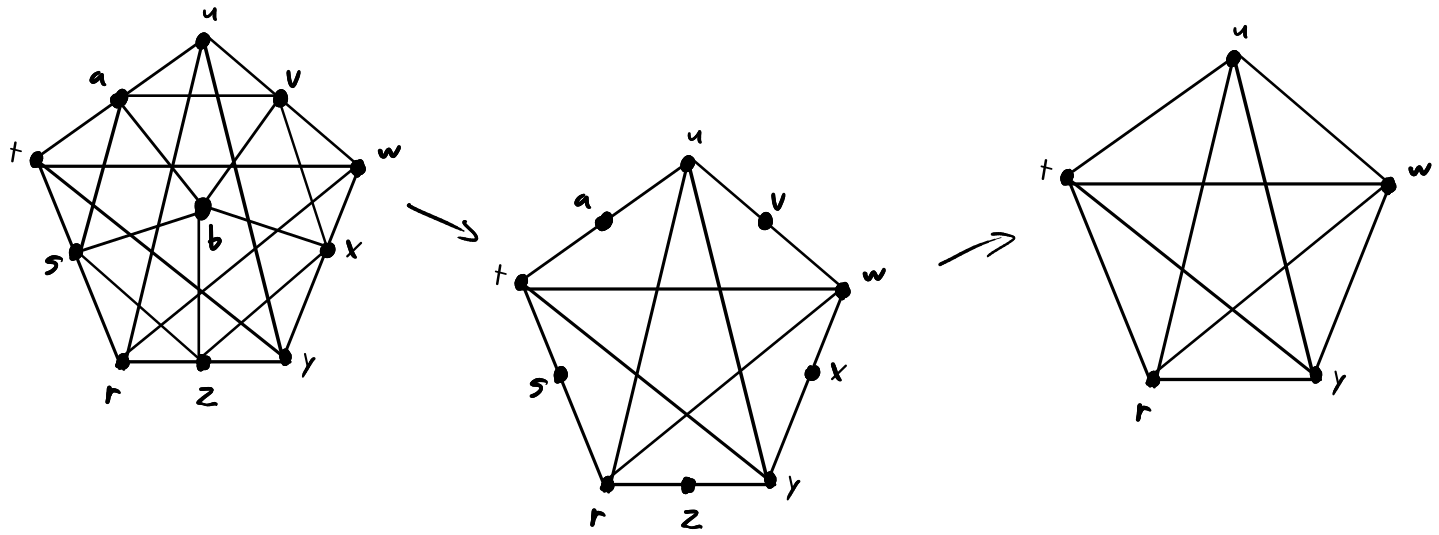
\includegraphics[scale=.5]{910.png}\end{center}
        Thus, by Kuratowski's Theorem, the graph of Figure 9.16 is nonplanar.
\end{proof}

\newpage\noindent\textbf{9.16} Proposition: There exist two non-isomorphic maximal planar graphs of the same order.
\begin{proof}
    Observe that the following two graphs are maximal planar because every region in each of them is triangular.
    Now, not that they have different degree sequences; the one on the left has a vertex of degree 5, but the one on the right has only vertices of degree 4.
    Thus, the two are not isomorphic.
\end{proof}

\newpage\noindent\textbf{9.18} Proposition: For each maximal planar graph $G$ of order $n\geq 3$, $\overline G$ is not maximal planar.
\begin{proof}
    Observe that the size of a maximal planar graph of order $n \geq 3$ is $3n - 6$.
    This follows directly from Theorem 9.2.
    Let $G$ be a maximal planar graph of order $n \geq 3$.
    Then, $G$ has size $3n-6$.
    Thus, $\overline G$ has size
    \begin{align*}
        {n \choose 2} - (3n-6) &= \frac{n(n-1)}2-3n+6 \\
                               &= \frac{n^2-n-6n+12}2 \\
                               &= \frac12n^2-\frac72n+6.
    \end{align*}
    Note that $\frac12x^2-\frac72x+6 = 3x-6$ only when $x=\frac12(13\pm\sqrt{73})$.
    Thus, when $x=n$, the two expressions are not equal.
    Therefore, $\overline G$ does not have $3n-6$ edges, so $\overline G$ is not maximal planar.
\end{proof}


\end{document}
